
\section{Future Work}
\label{sec:future}
Because of the nature of SINATRA, it is expected for there to be a large amount of future work. A critical part of SINATRA is that it will be developed into a state-of-the-art homegrown code which Cal Poly can use to help develop new aerospace technology.

\subsection{Boundaries}

One part of SINATRA which is underdeveloped is the handling of boundaries. Currently, SINATRA handles the main 6 boundaries of a cube. It has the capability to define the type of wall and the characteristics of the particles flowing through that wall. However, it ignores any boundaries inside of the domain, cannot break a boundary into multiple sections. While dealing with boundaries inside the domain will not be needed for a plasma plume, it will be important to be able to split the boundaries so that part of the wall can simulate the thruster nozzle. The path forward for boundaries is twofold. First, a boundary class needs to be built within SINATRA which allows the user to specify sections which will be different from the rest of the domain. At that stage it would be reasonable to simulate a thruster nozzle. \par

\indent The next stage would be to build Cart3D\textsuperscript{TM} integration. Cart3D\textsuperscript{TM} is a meshing software that can create an octree mesh which includes internal domain boundaries. This allows a user to import a Computer-aided design (CAD) file and get out a mesh which SINATRA can understand. This is critical for upper atmosphere calculations around aircraft or spacecraft bodies. It can also be used for objects in Low Earth Orbit. The Cart3D\textsuperscript{TM} tool will allow users to specify what each external and internal boundary type is and is able to split these boundaries into much smaller pieces. Cart3D\textsuperscript{TM} can also dynamically change the mesh size depending on distance to a wall and other user specifications which will allow for more accurate DSMC-PIC simulation data. This integration will need to be completed before SINATRA can create useful simulation results. The future researchers can also choose a difference meshing software depending on future requirements. \par


\subsection{Electric Thruster}

As mentioned above, in order for an accurate electric thruster simulation, there will need to be changes in how boundaries are handled in SINATRA. Updating the boundaries is the most important change that will be needed for accurate simulations of electric thruster plumes. The Poisson equation solver would need to be upgraded as well. Currently, a finite volume solver is being used. This is a robust solver which is well-researched and understood, but it has a few restrictions. First, and most importantly, the solver expects the mesh to be evenly sized across the entire domain. This works with the current version of SINATRA's home-built meshing software; however, once the mesh is not completely uniform, the Poisson solver will break. This solver can only handle straight boundaries, which is acceptable because the DSMC portion uses straight approximations of curves through the octree mesh. There are many other options for a Poisson solver that have been explored in PIC research. For example, the conjugate gradient solver might be a good option for SINATRA. Conjugate difference requires a symmetric positive definite matrix which the Finite Difference method creates \cite{FD_GS}. This upgrade would also greatly reduce the execution time, and therefore allow for larger and more accurate simulations. \par

% TO DO talk about the solver - using sparce matrices, handling the difference between cells and nodes, and changing solver
\subsection{Charged Particles}

There are many facets to simulating charged particles. While the author has captured the largest features, there are many other physical attributes which make charged particles a complicated and interesting subject. There are two main physical properties which would be the most likely candidates to be added to SINATRA. They are charged collisions and surface interactions. \par

\indent When charged particles are involved, there are many new types of particle collisions. Some types are ionization and recombination collisions. These are being ignored in SINATRA because the electrons are being modeled as a fluid. However, if magnetic fields were to be included, for example for a magnetic nozzle, or if the grids of an ion thruster need to be modeled, then the fluid assumption would no longer be valid. The simulation would have to drastically reduce its simulation time-step for the fast electrons and also need to consider ionization and recombination collisions. There are also chemical interactions that are also not being considered in the scope of this project. Both of those types of collisions will most likely not be needed for accurate plasma plume simulations. In order for these collisions to be included, the collision class will need to be updated to be able to handle multiple schemes within the same simulation. \par

\indent However, charge exchange collisions will need to be included eventually. Charge exchange collisions are instances where the electron orbital cloud of an ion and a neutral particle will interact \cite{pic_generic}. There is a possibility in these collision for an electron to be stripped from the neutral atom and become attached to the charged ion. The charge is exchanged between the two particles; the neutral atom becomes a charged ion and the charged ion becomes a neutral atom. However, there is no significant change in momentum. This type of collision is common and significant in electric thruster plumes. While most thrusters are efficient at ionizing the propellant, there are still neutral atoms which come out of the chamber and into the plume. Their relatively low velocities cause the relative density of the neutral atoms to be high near the thruster nozzle. Charge exchange collisions (CEX) are therefore likely. The resulting slow-moving ions are very susceptible to the radial component of the electric field set up by the plume. While the fast-moving ions will diverge, they do so at a low angle because of their high initial velocity. However, these new ions are moving slowly and therefore are more easily affected by the radial electric field. They create what is called CEX wings, seen in Figure \ref{fig:CEX} \cite{cex_wings}. This radial direction of charged ions can cause major interactions with the spacecraft including contamination, sputtering, and spacecraft charging. Therefore CEX interactions should be included when doing full spacecraft analysis. 


\begin{figure}
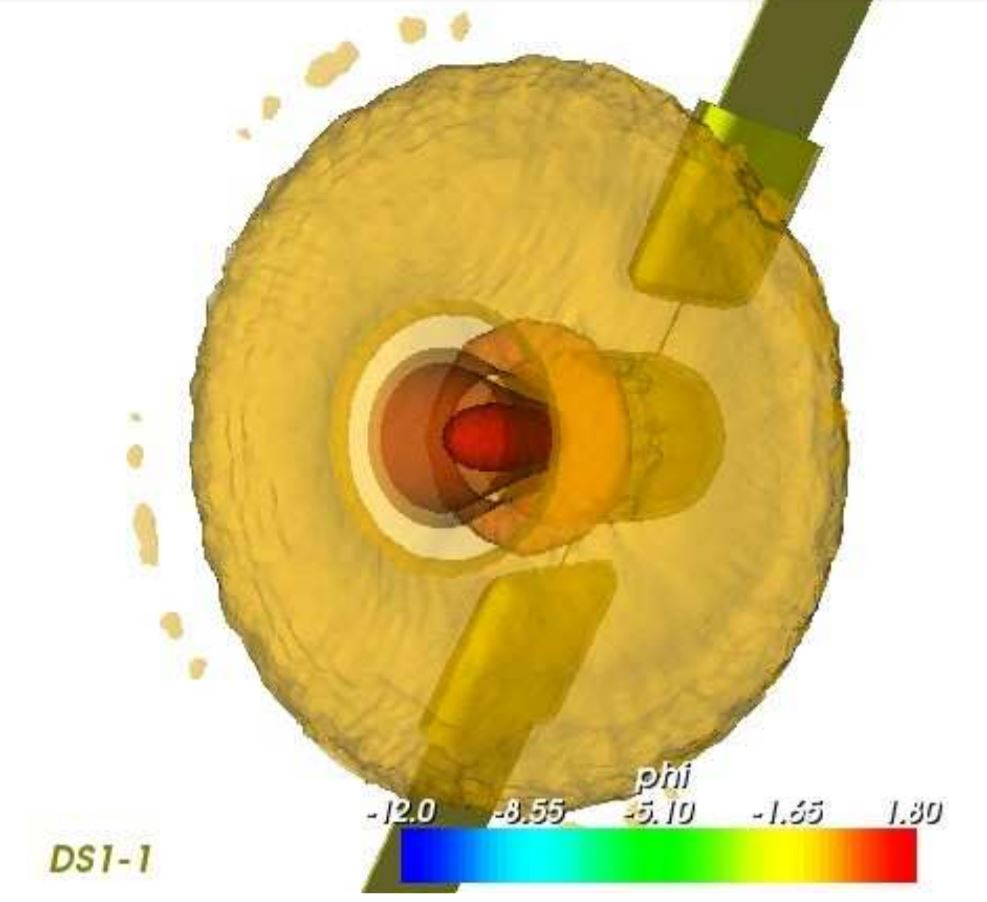
\includegraphics[width=.65\textwidth]{CEX.JPG}
\centering
\caption[Visualization of CEX wings]{Visualization of CEX wings \cite{cex_wings}}
\label{fig:CEX}
\end{figure}

\indent Another important quality of charged particles is their surface interactions. When high energy particles collide with metal surfaces they sputter off material and degregate the surface. This is an important design consideration in spacecraft with electric propulsion. SINATRA models various types of surface interactions through its boundary handling. There can be inflow, outflow, specular and diffuse walls. However, especially with CEX collisions, charged particles can interact with a spacecraft surface and impart their charge onto it \cite{surface_charge}. The surface can be modeled as a grounded conductor or as a perfect insulator or as a mix between the two. This type of modeling will need to be included into SINATRA whenever boundaries are introduced into the domain.

\subsection{SINATRA Efficiency and Capability}
\label{sec:auto_mesh}
There are many sections in SINATRA that need to be updated before SINATRA can be used as a cutting edge research tool. It was developed by mechanical and aerospace engineers, not by computer scientists. Therefore, many of the algorithms, storage methods, and memory access are not optimized. The author has removed the largest and simplest bottlenecks, but there are other areas that need to be optimized. The next largest bottleneck is the sampling of data. When SINATRA samples data from the simulation, it prints out text files. This printing is one of the slowest portions of the simulation. Tecplot\textsuperscript{TM} has an API which allows users to print binary files and Tecplot is able to input those binary files. This was attempted by the original developers, but they were not successful. It requires a deeper understanding of C++ and binary. There are many examples of possible optimization throughout the code which can be fixed by a developer with that type of skill set. It may also be possible to switch to the Visualization Toolkit VTK which has other features which may make sampling data much simpler and quicker. \par

\indent Within a computer scientist skill set lies parallelization. Similar to the bottlenecks above the author has implemented a simple version of parallelization; however, there are many better ways to implement it. It could be implemented by splitting the domain into multiple pieces, which is a possibility on account of the regularity of the octree mesh. However, this may not be the best option because particles must be transferred between the domains which is very computationally expensive. Another option would be to split a larger section of each time-step into many parts. The simulation could also be parallelized by having each core run the same simulation. Then the multiple different simulations could be averaged as a way to reduce the randomness of DSMC so that an accurate solution is calculated. Parallelization techniques are still on the cutting edge of computer science, and therefore this would be a fruitful project for a developer with experience in this area. \par

\indent Within the DSMC community, there are many schools of thought about the best way to work with time-steps and mesh sizes \cite{bird_dsmc}. It is possible to have variable time-steps as well as variable mesh sizes. It is also possible for the time-step to change for each particle depending on their velocity and the size of the mesh cell they are within. There are algorithms which create a mesh which changes cell size depending on the average number of particles in a cell. This creates a mesh which changes with the flow and eventually sets up an optimal mesh for that steady state flow condition. \par

\indent SINATRA is currently at its first iteration; therefore it uses a fixed time-step for all particles and a fixed mesh. Upgrading SINATRA to a more complicated time-step and mesh algorithm would be a good project for a future developer. In order to keep charged particle capability, the Poisson solver would have to be upgraded at the same time because it is currently based on the fixed mesh. This upgrade could greatly reduce SINATRA's execution time; therefore, it would allow higher resolution and accurate simulations. It would be beneficial to implement a user choice for different Poisson solvers so that a user can compare various solvers and use their various advantages depending on their simulation requirements. It would also be useful to include an option for the user to have SINATRA assume a linearized Boltzmann equation, which assumes that \(n_i-n_e << n_i\). This would allow a much quicker calculation of the potential and be a good low accuracy solver for the beginning stages of complicated simulations.  \par

\indent The stencil implementation will also need to be upgraded. When non-uniform Cartesian grids are included in SINATRA the stencil implementation will fail. The Finite Difference Method requires an uniform mesh. However, the Finite Volume method may be a good alternative to be used for the new mesh types. It will need to be upgraded to be much more robust to accommodate complicated meshes. The stencil implementation can also be upgraded. Currently the sparse matrix wastes a large amount of computing power through having a large empty matrix and multiplying many zeros. This can be improved thorough either sparse matrix calculations or by calculating the required row of the matrix only when going to do operations upon it. Finally, the future developers will need to be careful when using a non-uniform Cartesian grid and depositing charge on account of the octree structure. \par

\indent Another area of possible improvement is within the octree search algorithm. Future developers will need to start with confirming that the current search algorithm fits the expected \(n log(n)\) order where n is the number of items in the search. Once confirmed other advanced algorithms can be implemented including aligning the octree mesh to an integer system so that the integer positions can be used as inputs into the data matrix within the calculations. \par

\subsection{Systems Operations}

It will be important to continually update the systems engineering sections of SINATRA. The author has set up systems which will hopefully be helpful at keeping SINATRA up-to-date and relevant, but they will need to be monitored and maintained
 \par

\indent First, the simple distributions need to be kept up-to-date. There are distributions for Windows, Linux, and Mac. If SINATRA continues to grow at Cal Poly, an official release website with version control can be set up. Until then it will be released through .zip files being sent to the new user; therefore, the distributions need to be up-to-date with the current stable version of SINATRA, input files, and the GUI. \par

\indent The GUI will also need to be updated as there are changes to the input class. Whenever the input class requires a different way to input variables to the simulation, the GUI will also need to be changed to accommodate for those changes. It will also have to be updated when the boundary class or output class changes their user interface. It is not difficult to keep the GUI up-to-date, but it can easily become obsolete if it is left alone during further development. \par

\indent The author has ensured that the GitHub\textsuperscript{\textregistered} repository is kept clean and up-to-date as much as possible. It will be necessary to use the GitHub\textsuperscript{\textregistered} repository while developing new code. One pitfall could be that new developers only develop on their local machines and ignore the GitHub\textsuperscript{\textregistered} repository. This habit could ruin the continuity of the version control of GitHub\textsuperscript{\textregistered} and more importantly could make it harder for new developers to add their contributions. The GitHub\textsuperscript{\textregistered} should be kept as a version of the code which can be easily shared with new developers, so they are not be confused nor distracted by extra files and information. If SINATRA is well taken care of, it will become a legacy code that will allow Cal Poly to shine as a school with advanced modeling skills and allow new and revolutionary technology to come from ``Learning by Doing".




